% -*- latex -*-
%%%%%%%%%%%%%%%%%%%%%%%%%%%%%%%%%%%%%%%%%%%%%%%%%%%%%%%%%%%%%%%%
%%%%%%%%%%%%%%%%%%%%%%%%%%%%%%%%%%%%%%%%%%%%%%%%%%%%%%%%%%%%%%%%
%%%%
%%%% This text file is part of the source of 
%%%% `Parallel Programming in MPI and OpenMP'
%%%% by Victor Eijkhout, copyright 2012-2021
%%%%
%%%% mpi.tex : leftover MPI topics
%%%%
%%%%%%%%%%%%%%%%%%%%%%%%%%%%%%%%%%%%%%%%%%%%%%%%%%%%%%%%%%%%%%%%
%%%%%%%%%%%%%%%%%%%%%%%%%%%%%%%%%%%%%%%%%%%%%%%%%%%%%%%%%%%%%%%%

\Level 0 {Bandwidth and halfbandwidth}

Bandwidth is the quantity that measures the number of bytes per second that
can go through a connection.
This definition seems straightforward, but commes with many footnotes.
\begin{itemize}
\item The size of the message used matters, since there is a \indexterm{latency}
  cost to merely starting the message. Often, the bandwidth number quoted
  is an asymptotic figure, hard to achieve in practice.
\item If a certain bandwidth figure is attained between a pair of processes,
  will two pairs, sending simultaneously, reach the same number?
\item Does the bandwidth depend on the choice of processes to measure?
\item And combinations of these considerations.
\end{itemize}

A useful measure comes from asking what bandwdith is achievable if all processes
are either sending or receiving.
As a further refinement, we ask what the least favorable choice is
for the communicating pairs:
\begin{quote}
  Halfbandwidth is defined as the minimum total bandwidth,
  over all possible choices of splitting the processes into
  a sending and receiving half.
\end{quote}

\begin{figure}[ht]
  \hbox\bgroup  %pyskip
  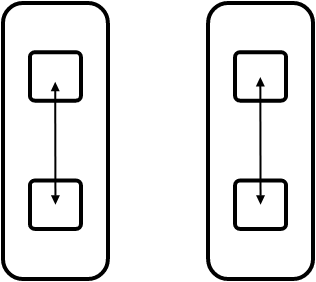
\includegraphics[scale=.4]{hbwprocs-intra}
  \hss  %pyskip
  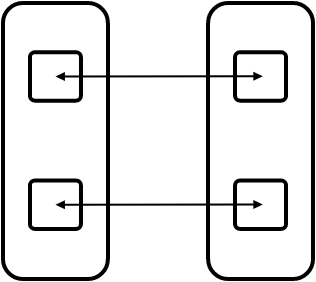
\includegraphics[scale=.4]{hbwprocs-inter}
  \hss  %pyskip
  \egroup  %pyskip
  \caption{Intra and inter schemes for bandwidth}
  \label{fig:interintra}
\end{figure}

Figure~\ref{fig:interintra} illustrates the `intra' (left)
and `inter' (right) scheme for letting all processes
communicate in pairs.
With intra-communication, the messages do not rely on the network
so we expect to measure high bandwidth.
With inter-communication, all messages go through the network
and we expect to measure a lower number.

However, there are more issues to explore,
which we will now do.

First of all we need to find pairs of processes.
Consecutive pairs:
\cxxverbatimsnippet{procpairclose}
Pairs that are $P/2$ apart:
\cxxverbatimsnippet{procpairspread}

\begin{figure}[ht]
  \pgfplotsset{width=3.5in,compat=1.7}
  \hbox\bgroup %pyskip
  \tikzsetnextfilename{hbw-intra}
  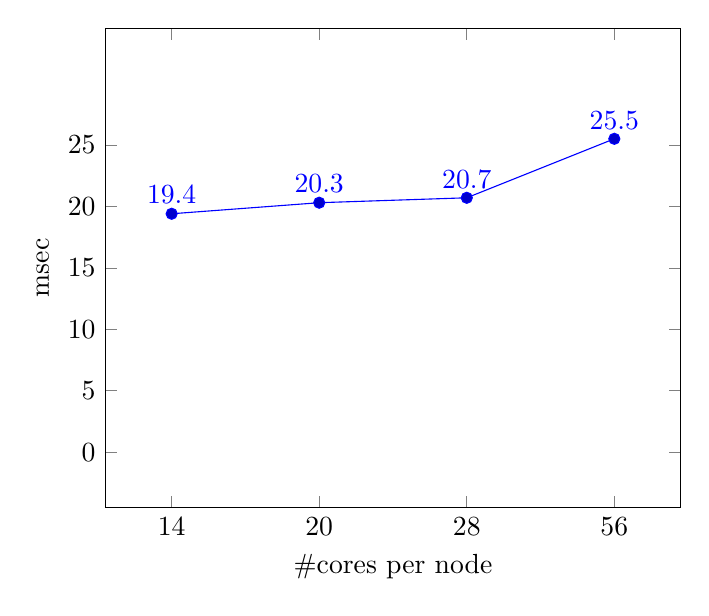
\begin{tikzpicture}  
    \begin{axis}
      [  
        enlargelimits=0.15,
        xlabel={\#cores per node},
        ylabel={msec}, ymin=0, ymax=30,
        symbolic x coords={14,20,28,56},
        xtick=data,  ytick={0,5,10,15,20,25},
        nodes near coords,  
        nodes near coords align={vertical},  
      ]  
      \addplot coordinates {(14, 19.4) (20, 20.3) (28, 20.7) (56, 25.5) };
      %\legend{milliseconds per pingpong}
    \end{axis}
  \end{tikzpicture}  

  \tikzsetnextfilename{hbw-inter}
  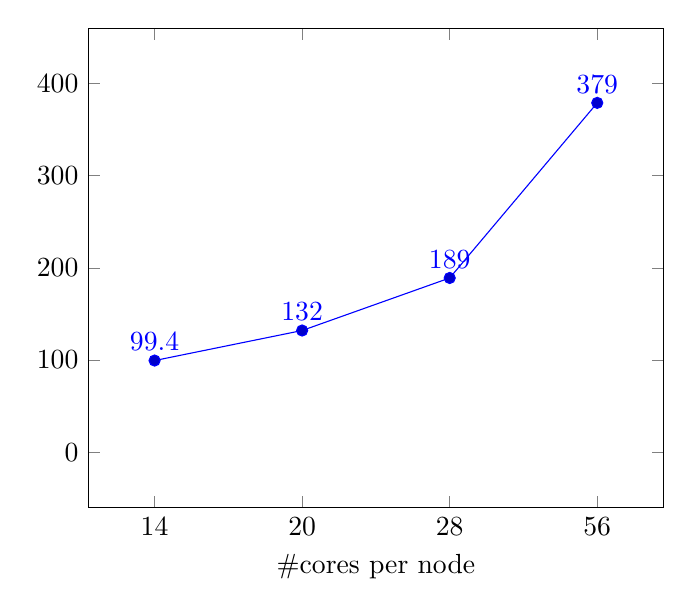
\begin{tikzpicture}  
    \begin{axis}
      [  
        enlargelimits=0.15,
        xlabel={\#cores per node},
        symbolic x coords={14,20,28,56},
        xtick=data,  ytick={0,100,200,300,400}, ymin=0, ymax=400,
        nodes near coords,  
        nodes near coords align={vertical},  
      ]  
      \addplot coordinates {(14, 99.4) (20, 132) (28, 189) (56, 379) };
      %\legend{milliseconds per pingpong}
    \end{axis}
  \end{tikzpicture}  
  \egroup %pyskip
  \caption{Time as a function of core count. Left: on node. Right: between nodes.}
  \label{fig:hbw-interintra}
\end{figure}

The halfbandwidth is measured as the total number of bytes sent
divided by the total time.
Both numbers are measured outside a repeat loop that does each
transaction 100~times.
%
\cxxverbatimsnippet{hbwmeasure}

In the left graph of figure~\ref{fig:hbw-interintra} we see that the time
for $P/2$ simultaneous pingpongs stays fairly constant.
This reflects the fact that, on node, the ping pong operations are
data copies, which proceed simultaneously.
Thus, the time is independent of the number of cores that are moving data.
The exception is the final data point: with all cores active we take up
more than the available bandwidth on the node.

In the right graph, each pingpong is inter-node, going through the network.
Here we see the runtime go up linearly with the number of pingpongs,
or somewhat worse than that.
This reflects the fact that network transfers are done sequentially.
(Actually, message can be broken up in packets, as long as they
satisfy MPI message semantics. This does not alter our argument.)

\begin{comment}
  \begin{figure}
    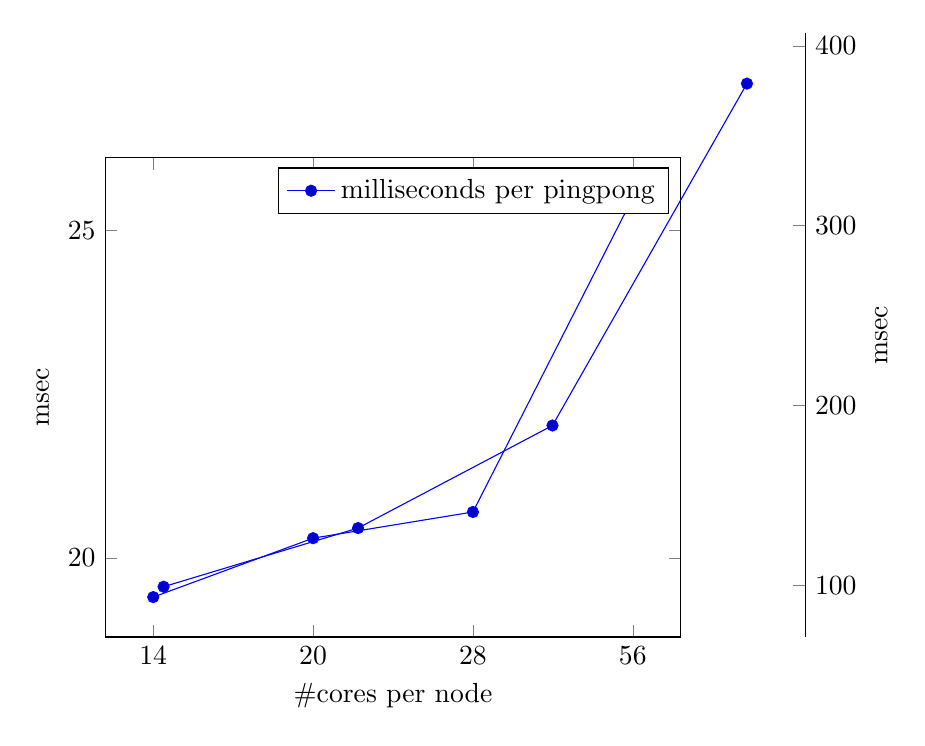
\begin{tikzpicture}  
      \begin{axis}
        [  
          xlabel={\#cores per node},
          ylabel={msec},
          symbolic x coords={14,20,28,56},
          xtick=data,  ytick={0,5,10,15,20,25},
          %nodes near coords,  
          %nodes near coords align={vertical},  
        ]  
        \addplot coordinates {(14, 19.4) (20, 20.3) (28, 20.7) (56, 25.5) };
        \legend{milliseconds per pingpong}
      \end{axis}

      \begin{axis}
        [  
          ylabel={msec},
          scale only axis,
          symbolic x coords={14,20,28,56},
          xtick=data,  ytick={0,100,200,300,400},
          axis y line*=right,
          axis x line=none,
        ]  
        \addplot coordinates {(14, 99.4) (20, 132) (28, 189) (56, 379) };
      \end{axis}
    \end{tikzpicture}  
    \caption{Timing for pingpong between nodes}
    %\label{fig:omp-speed-hyper}
  \end{figure}
\end{comment}

\begin{comment}
\begin{verbatim}
using buffer of size 100000 (doubles)

================================================================
Strategy 1 ran in     25483 usec for 11200 pingpongs evaluating to halfbandwidth 3.52e+11 byte/sec
Strategy 2 ran in    379679 usec for 11200 pingpongs evaluating to halfbandwidth 2.36e+10 byte/sec
================================================================

using only processes modulo 2
================================================================
Strategy 1 ran in     20742 usec for 5600 pingpongs evaluating to halfbandwidth 2.16e+11 byte/sec
Strategy 2 ran in    189442 usec for 5600 pingpongs evaluating to halfbandwidth 2.36e+10 byte/sec
================================================================

using only processes modulo 3
================================================================
Strategy 1 ran in     20317 usec for 3800 pingpongs evaluating to halfbandwidth 1.50e+11 byte/sec
Strategy 2 ran in    131933 usec for 3800 pingpongs evaluating to halfbandwidth 2.30e+10 byte/sec
================================================================

using only processes modulo 4

================================================================
Strategy 1 ran in     19391 usec for 2800 pingpongs evaluating to halfbandwidth 1.16e+11 byte/sec
Strategy 2 ran in     99462 usec for 2800 pingpongs evaluating to halfbandwidth 2.25e+10 byte/sec
================================================================
\end{verbatim}
\end{comment}

\begin{figure}
  \pgfplotsset{width=3.5in,compat=1.7}
  \hbox\bgroup %pyskip
  \tikzsetnextfilename{hbw-intra-bw}
  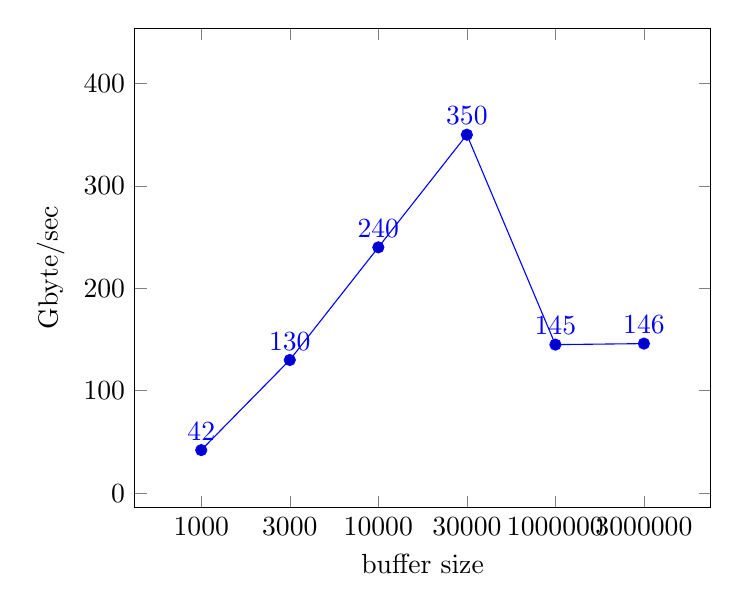
\begin{tikzpicture}  
    \begin{axis}
      [  
        enlargelimits=0.15,
        xlabel={buffer size},
        ylabel={Gbyte/sec}, ymin=40, ymax=400,
        symbolic x coords={1000, 3000, 10000, 30000, 1000000, 3000000},
        xtick=data,
        nodes near coords,  
        nodes near coords align={vertical},  
      ]  
      \addplot coordinates {(1000, 42) (3000, 130) (10000, 240) (30000, 350) (1000000, 145) (3000000, 146)};
      %\legend{milliseconds per pingpong}
    \end{axis}
  \end{tikzpicture}  

  \tikzsetnextfilename{hbw-inter-bw}
  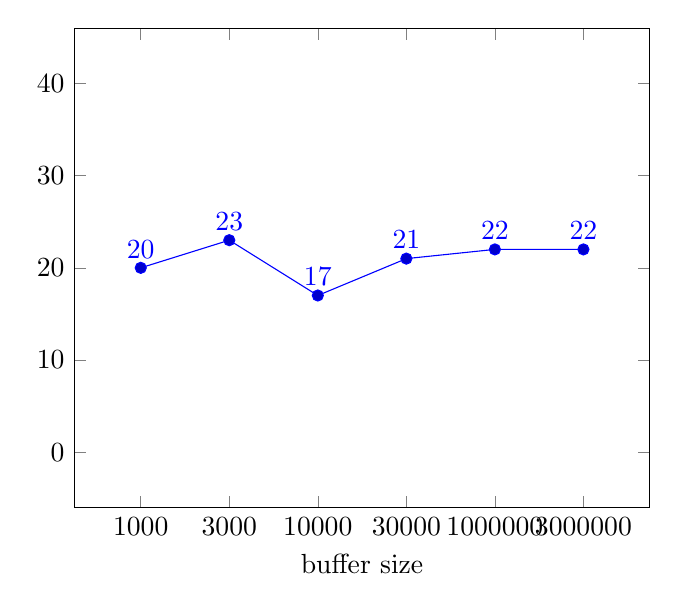
\begin{tikzpicture}  
    \begin{axis}
      [  
        enlargelimits=0.15,
        xlabel={buffer size},
        symbolic x coords={1000, 3000, 10000, 30000, 1000000, 3000000},
        xtick=data,  ymin=0, ymax=40,
        nodes near coords,  
        nodes near coords align={vertical},  
      ]  
      \addplot coordinates {(1000, 20) (3000, 23) (10000, 17) (30000, 21) (1000000, 22) (3000000, 22)};
      %\legend{milliseconds per pingpong}
    \end{axis}
  \end{tikzpicture}  
  \egroup %pyskip
  \caption{Bandwidth as a function of buffer size. Left: on node. Right: between nodes.}
  \label{fig:hbw-interintra-b}
\end{figure}

Next we explore the influence of the buffer size on performance.
The right graph in figure~\ref{fig:hbw-interintra-b}
show that inter-node bandwidth is almost independent of the buffer size.
This means that even our smallest buffer is large enough to overcome
any MPI startup cost.

On other hand, the left graph shows a more complicated pattern.
Initially, the bandwidth increases, possibly reflecting
the decreasing importance of MPI startup.
For the final data points, however, performance drops again.
This is due to the fact that the data size overflows
cache size, and we are dominated by bandwidth from memory, rather than cache.


\begin{comment}
\begin{verbatim}
[c205-025 cxx:6] make halfbandwidth && for s in 1000 3000 10000 30000 1000000 3000000 ; do ibrun halfbandwidth -m 2 -s $s ; done | grep -v TACC
make: `halfbandwidth' is up to date.
Strategy 1 ran in      1078 usec for 5600 pingpongs evaluating to halfbandwidth 4.16e+10 byte/sec
Strategy 2 ran in      2244 usec for 5600 pingpongs evaluating to halfbandwidth 2.00e+10 byte/sec
================================================================
Strategy 1 ran in      1038 usec for 5600 pingpongs evaluating to halfbandwidth 1.29e+11 byte/sec
Strategy 2 ran in      5972 usec for 5600 pingpongs evaluating to halfbandwidth 2.25e+10 byte/sec
================================================================
Strategy 1 ran in      1872 usec for 5600 pingpongs evaluating to halfbandwidth 2.39e+11 byte/sec
Strategy 2 ran in     25846 usec for 5600 pingpongs evaluating to halfbandwidth 1.73e+10 byte/sec
================================================================
Strategy 1 ran in      3848 usec for 5600 pingpongs evaluating to halfbandwidth 3.49e+11 byte/sec
Strategy 2 ran in     63529 usec for 5600 pingpongs evaluating to halfbandwidth 2.12e+10 byte/sec
================================================================
Strategy 1 ran in    308869 usec for 5600 pingpongs evaluating to halfbandwidth 1.45e+11 byte/sec
Strategy 2 ran in   2049570 usec for 5600 pingpongs evaluating to halfbandwidth 2.19e+10 byte/sec
================================================================
Strategy 1 ran in    921737 usec for 5600 pingpongs evaluating to halfbandwidth 1.46e+11 byte/sec
Strategy 2 ran in   6173416 usec for 5600 pingpongs evaluating to halfbandwidth 2.18e+10 byte/sec
\end{verbatim}
\end{comment}
